\section{Dependency Hell}
Il software che scriviamo ha un sacco di dipendenze (libreria di sistema, ecc.). Il software che si scrive non è mai tutto sotto il nostro controllo (non è solo il codice che scriviamo); le nostre istruzioni si appoggiano a moltissime altre che non sono sotto al nostro controllo.
\\\\ Qualsiasi applicazione dipende da componenti software fuori dal controllo del produttore: kernel, device driver, librerie di sistema, librerie di supporto. 
\\ Anche una semplice applicazione deve interagire con le librerie messe a disposizione dal S.O.
Ad esempio la calcolatrice di gnome ha 83 dipendenze.
\\\\ Le dipendenze creano problemi, vogliamo cercare di essere indipendenti. 
\\\\ Troviamo il concetto di \textbf{dependency hell}: le dipendenze rischiano di sfuggirmi di mano, ovvero perdo il controllo delle dipendenze. Io dipendo da cose che cambiano senza che me ne accorga e l'applicazione non funziona più.
\\\\
Questo concetto va sicuramente meglio con i linguaggi interpretati: alle dipendenze di sistema generalmente sopperisce l’interprete (ma non sempre: con la macchina virtuale Java per esempio può essere piuttosto faticoso utilizzare specifiche librerie grafiche).
\begin{itemize}
    \item un'applicazione usa librerie per non "reinventare la ruota"
    \item evitare la sindrome NIH (Not invented here): i programmatori diffidano da cose che non hanno sviluppato loro. Sovraccarica troppo il gruppo di lavoro e nasce dall'esigenza di non dipendere troppo.
    \item evitare le dipendenze inutili
\end{itemize}
Le dipendenze vanno il più possibile esplicitamente documentate e motivate.
\\\\ 
Abbiamo già discusso che distributori come Debian devono gran parte del loro successo alla ricca documentazione delle dipendenze:
\begin{itemize}
    \item ogni pacchetto è regolato da un control file, che specifica le caratteristiche 
    \item le dipendenze: Depends, Recommends, Suggests, Enhances, Pre-Depends 
    \item gli script da eseguire per mantenere l’integrità del sistema: preinst, postinst, prerm, postrm
    \item la priorità: Required, Important, Standard, Optional, Extra
\end{itemize}
Il problema esiste non solo a livello di sistema, ma anche di singola applicazione (DLL hell):
\begin{itemize}
    \item Riproducibilità
    \item Ambienti di “scripting” per i quali non sono possibili compilazioni “statiche”
    \item Gestione di installazioni concorrenti di diverse versioni
\end{itemize}
\subsubsection{Python}
Esaminiamo il caso di Python, ma considerazioni analoghe valgono ormai per moltissime piattaforme di sviluppo (npm, stack, ...)
Onnipresenti poi i sistemi di distribuzione centralizzata:
\begin{itemize}
    \item PHP Pear
    \item CPAN Perl 
    \item CTAN Tex 
    \item MELPA Emacs
    \item ....
\end{itemize}
Python fornisce un meccanismo standard per documentare le dipendenze di un'applicazione:

\begin{minted}[bgcolor=LightGray, fontsize=\footnotesize]{Python}
from setuptools import setup

setup(
    name="MyLibrary",
    version="1.0",
    install\_requires=[
    "requests",
    "bcrypt",
    ],
    # ...
)
\end{minted}
Esistono poi dei punti di distribuzione centralizzata: per esempio PYPI e naturalmente un package manager: 
\textbf{pip install requests}, installa la libreria request nel mio sistema (sovrascrivendo quella vecchia se presente, creando problemi ai programmi che usavano la versione vecchia).
\\\\ Cosa succede se c'era già la libreria request? Viene fatto un upgrade, ma posso avere un'applicazione che dipendeva dalla versione vecchia e che ora non funziona più.
\\\\ Come posso fare per installare più versioni delle librerie?
Con sistemi come virtualenv non viene più installata la libreria a livello di sistema ma può essere installata a livello di utente, a livello della singola directory o a livello di sistema. 
\\\\ Sempre più spesso non vogliamo installazioni "system-wide", ma "user-wide" o addirittura "application specific".
\begin{minted}[bgcolor=LightGray, fontsize=\footnotesize]{bash}
$ cd ~/usr/local/src/app/
$ virtualenv env
New python executable in env/bin/python
Installing setuptools............done.
Installing pip...............done.
$ pip ....
$ python ....
\end{minted} 
(Con source ./env/activate si pu`o semplificare la chiamata dei programmi)
\\\\ virtualenv funziona nel seguente modo (guardando il codice precedente: 
\begin{itemize}
    \item richiama virtualenv che crea una directory di nome "env" dove mette tutto ciò che serve per permettere all'applicazione di funzionare
    \item virtualenv va attivato, quindi mettere nel path le directory dove ha installato i vari programmi in modo tale che poi quando viene eseguito un comando python, non viene eseguito il python del sistema, ma quello dello specifico virtualenv
\end{itemize}
Come garantisco l'esplicitazione delle dipendenze?
\begin{minted}[bgcolor=LightGray, fontsize=\footnotesize]{bash}
$ pip install pippo
$ pip freeze > requirements.txt
$ pip install -r requirements.txt
\end{minted} 
pip tiene traccia anche delle cose che ho installato.
pip freeze $>$ file.txt : salva in file.txt le librerie che sono già installate nella macchina.
Esempio: 
\\ python3 -m virtualenv PLUTO : installa nella dir PLUTO il virtual enviroment. 
\\ pip install non scarica solo la libreria ma anche le dipendenze della libreria stessa a cui fa riferimento.

\\\\ \noindent \textbf{Problemi}
\begin{itemize}
    \item Può non essere banale tenere aggiornato un virtualenv/pipenv
    \item Source distribution vs. Wheel (egg)
    \item Moltissime duplicazioni virtualenvwrapper
    \item Sistemi più generali, cross-platform: conda
\end{itemize}

\noindent Utilizziamo il versionamento semantico: uno standard per dare i nomi di versioni. Si basa su 3 token: MAJOR.MINOR.PATCH
\begin{itemize}
    \item MAJOR cambia quando ci sono cambiamenti incompatibili nelle API
    \item MINOR cambia con nuove funzionalità (backwards-compatibile)
    \item PATCH solo bugfix
\end{itemize}
L'uso di questo meccanismo aiuta i package manager e permette di fare cose più sofisticate.

\section{Sistemi di build automation}
Costruire un prodotto software fatto di molti componenti è tutt'altro che banale:
\begin{itemize}
    \item dipendenze da componenti che non controlliamo (dependency hell)
    \item dipendenze fra componenti che stiamo sviluppando
\end{itemize}

\subsection{Make}
Make (1977) è nato per ottimizzare tempi di compilazione.
Permette di specificare dipendenze fra processi di generazione.\\
Dipendenze: se cambia (secondo la data dell'ultima modifica) un prerequisito, allora il processo di generazione deve essere ripetuto.

\begin{minted}[bgcolor=LightGray, fontsize=\footnotesize]{make}
helloworld.o: helloworld.c
        cc -c -o helloworld.o helloworld.c 
helloworld: helloworld.o
        cc -o \$@ \$<
.PHONY: clean
clean:
    rm helloworld.o helloworld
\end{minted} 
Le regole (o ricette) del make file sono composte da:
\begin{itemize}
    \item target (in blu prima dei :)
    \item sorgente (dopo i :)
    \item comando 
\end{itemize}
.PHONY è un nome fasullo di target che mi serve per poter lanciare il comando corrispondente tramite make clean.\\
Make è un gestore di dipendenze a livello di processi. 
Le dipendenze definiscono un grafo aciclico che ammette un unico ordinamento topologico (in quanto si passa una sola volta da ogni target). I processi di generazione (ricetta) sono eseguiti seguendo l'ordinamento topologico.\\
Nei make moderni è possibile eseguire processi di generazione indipendenti in parallelo (make -j).\\
Il modello di make assume un ambiente di build fisso:
l’ipotesi è irrealistica perfino nel mondo dello sviluppo anni ’70 (C/UNIX): compilatori, librerie cambiano molto anche nell’ambito degli standard.\\
Ad esempio in C si hanno problemi di non portabilità dovuti a funzioni che non esistono ovunque, hanno nomi/prototipi/comportamenti diversi ecc...\\
Le soluzioni adottate sono:
\begin{itemize}
    \item \#if/\#else
    \item substitution macros
    \item substitution functions
\end{itemize}

\begin{minted}[bgcolor=LightGray, fontsize=\footnotesize]{c}
#if !defined(CODE_EXECUTABLE)
    static long pagesize = 0;
#if defined(EXECUTABLE_VIA_MMAP_DEVZERO)
    static int zero_fd;
#endif
    if (!pagesize) {
#if defined(HAVE_MACH_VM)
        pagesize = vm_page_size;
#else
        pagesize = getpagesize();
#endif
#if defined(EXECUTABLE_VIA_MMAP_DEVZERO)
        zero_fd = open("/dev/zero", O_RDONLY,0644);
        if (zero_fd < 0) {
            fprintf(stderr, "trampoline: Cannot open /dev/zero!\n");
            abort();
        }
#endif
    }
#endif
\end{minted} 

\subsection{Configure}
Il passo successivo è autoconf: è uno strumento che serve a limitare i difetti di make (si usa con make). Autoconf è una grande repository di regole tutte diverse. Produce uno script che si chiama configure, che non è altro che un tool di configurazione che prepara l'ambiente di sviluppo in modo da poter eseguire la build in un sistema diverso da quello in cui è stato creato, modificando il makefile.
\begin{figure}[H]
	\centering
	 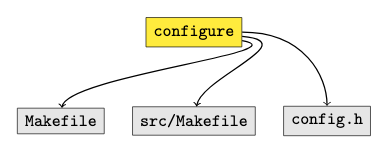
\includegraphics[scale=0.6]{img/config1.png}
\end{figure}
\noindent Con autoconf quindi produco uno script configure che se faccio andare prima di make, modifica Makefile nella maniera adeguata che possa poi essere compilato dal sistema. 
Make da solo è legato ad un ambiente fisso, uno scenario in cui tutte le persone che compilano il mio programma sullo stesso sitema, make funziona benissimo. 
Ho bisogno quindi che adatti la build all'ecosistema di sviluppo in cui mi trovo. Make gestisce quindi le dipendenze fra i processi di generazione, autoconf adatta le ricette all'ambiente di sviluppo in cui sto facendo la build. 

\begin{figure}[H]
	\centering
	 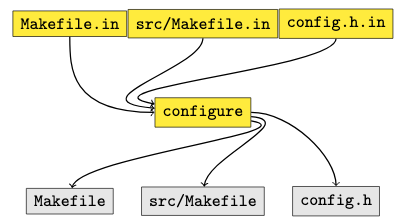
\includegraphics[scale=0.6]{img/config2.png}
\end{figure}

\noindent Autoconf e make fanno insieme un sistema di build automation. 
La build è composta da: 
\begin{itemize}
    \item gestione delle dipendenze
    \item processi di generazione (make)
    \item riconfigurazione all'ambiente di build
\end{itemize} 

\subsubsection{Ant}
In Java la build automation è organizzata tramite Ant. 
Ant è basato su XML. 

\begin{figure}[H]
	\centering
	 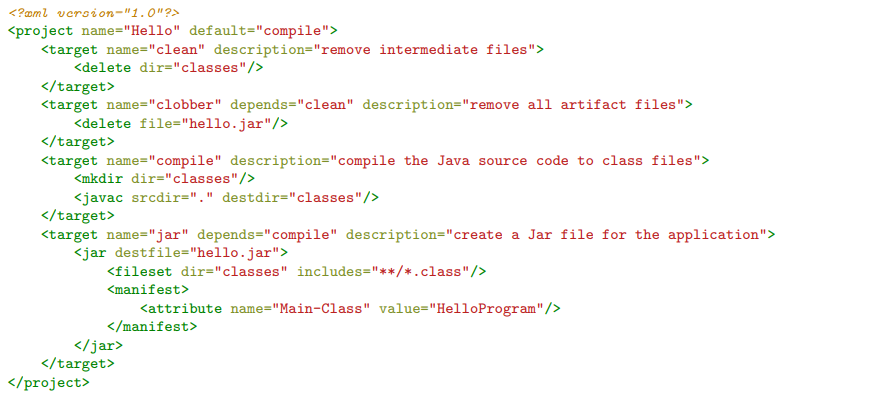
\includegraphics[scale=0.7]{img/ant.png}
\end{figure}

\noindent Prendiamo ad esempio il target "compile" le sue entità.
Le entità sono l'equivalente dei comandi, infatti prendiamo ad esempio mkdir: a differenza del makefile, non abbiamo il comando shell ma un'entità. 

\noindent Evita di dover adattare i processi di generazione per più sistemi. Se ho ant su Linux e su Windows sono sicuro che mkdir funziona sia su Linux che su Windows.
È pensato così per essere facilmente letto dalla macchina. 


\subsection{Gradle}
È un sistema che usa un linguaggio di Java chiamato Groovy. L'obiettivo è descrivere i processi di generazione di un software. 
Gradle è una descrizione in cui si mette il meno possibile, devo descrivere le peculiarità del mio progetto. Non dico che il compilatore di Java si chiama javac perchè una cosa normale, ma se il compilatore si dovesse chiamare pippo, allora devo dire questa cosa. Supporta il test e fa anche della reportistica: non solo genera il software ma fa dei log che ci dicono cos'è stato fatto. 

\subsection{Prospettiva}
\begin{itemize}
    \item \textbf{Make:} l'ambiente di sviluppo è implicito: ho solo le dipendenze tra gli artifact sotto controllo.
    \\ Tiene quindi traccia delle dipendenze tra i file di generazione e la limitazione è che assume un ambiente di sviluppo fisso. A make devo associare altre cose come autoconf, se voglio fare una vera build automation
    \item \textbf{Ant}: l'ambiente non è più dato per scontato ma costruisce i mattoni necessari ai processi di generazione. Nasce con in mente un ambiente di sviluppo che è quello di Java.
    Può sostituire gli elementi del processo di sviluppo con dei plugin. Non fa più l'assunzione di essere in un ambiente fisso
    \item \textbf{Gradle}: oltre a fare ciò che fa ant, permette di descrivere l'ambiente di sviluppo stesso. Quindi non solo ho la descrizione dei processi di generazione (come in make e ant), descrive anche sé stesso
\end{itemize}

\clearpage
\section{Documentazione dei componenti}
Strumenti che permettono di descrivere tutto il sapere implicito del singolo. Nell'ambito dell'ingegneria del software si parla di separation of concern: separazione/isolamento di problematiche diverse, in modo da riuscire a pensare ad una cosa alla volta e ad affidare una problematica ad un persona diversa. \\ Come si può suddividere il lavoro, senza la continua necessità di coordinazione? Perchè un sottogruppo di lavoro possa procedere in “isolamento” dovrebbe conoscere i componenti sviluppati da altri (o che altri svilupperanno), cioè conoscere il loro comportamento:
\begin{itemize}
    \item in situazioni fisiologiche(correttezza)
    \item in situazioni patologiche(robustezza)
\end{itemize}
A questo scopo è quindi necessario specificare il funzionamento del sistema.\\
\noindent Abbiamo parlato di correttezza e robustezza, ma esattamente cosa sono:\\\\
\textbf{Correttezza}: \begin{quote}
    "The degree to which a system or component is free from faults in its specification, design, and implementation"
\end{quote}
\textbf{Robustezza}: \begin{quote}
"The degree to which a system or component can function correctly in the presenceof invalid inputs or stressful environmental conditions."
\end{quote}

\noindent Una specifica è una descrizione delle proprietà del marchingegno/componente utilizzato per risolvere un problema (a sua volta definito dai requisiti di progetto). Le specifiche, perciò, sono una descrizione delle parti che compongono la soluzione: le modalità computazionali però sono lasciate impredicate.\\\\

\noindent Le specifiche costituiscono naturalmente l'interfaccia tra gruppi che si suddividono l'implementazione di un sistema complesso.
\begin{itemize}
    \item Il coordinamento rimane necessario a livello di specifica: ma accordarsi su cosa sembra più facile che sul come.
    \item I sottogruppi avranno la responsabilità di aderire alle specifiche nelle loro implementazioni.
\end{itemize}

\noindent Perry \& Evangelist (nel 1985) identificano una serie di“Interface Fault” cher imangono sostanzialmente comuni anche nei sistemi complessi di oggi.
\begin{itemize}
    \item Construction (mismatchinterface/implementation)
    \item Inadequate functionality
    \item Disagreements on functionality
    \item Misuse of interface
    \item Data structure alteration
    \item Violation of data constraints
    \item Initialization/value errors
    \item Inadequate error processing
    \item Inadequate postprocessing (resource deallocation)
    \item Inadequate interface support
    \item Changes/Added functionality
    \item Coordination of changes
    \item Timing/performance problems
\end{itemize}

\noindent Introduciamo quindi il meccanismo dell'asserzione che verifica che le ipotesi confermino il reale funzionamento del componente che sto sviluppando.\\\\
\textbf{Assert}: \begin{quote} "(1) a logical expression specifying a program state that must exist or a set ofconditions that program variables must satisfy at a particular point during programexecution.  (2) a function or macro that complains loudly if a design assumption onwhich the code is based is not true." \end{quote}
In pratica l'asserzione è l'esplicitazione di un requisito sotto forma di codice.

\noindent È utile ragionare su “pattern” di asserzioni, spesso codificati in assertion languages/libraries.
Descrive un preprocessore (APP) per produrre asserzioni:  il preprocessore lavora suspeciali “commenti” /*@@*/:
\begin{itemize}
    \item assume
    \item promise
    \item return
    \item assert
\end{itemize}
\clearpage
\begin{minted}[bgcolor=LightGray, fontsize=\footnotesize]{c}
int square_root(int x);
/*@ 
    assume x >= 0;
    return y where y >= 0;
    return y where y*y <= x 
    &&  x < (y+1)*(y+1); 
@*/

void swap(int* x, int* y);
/*@
    assume x && y && x != y;
    promise *x == in *y;
    promise *y == in *x;
@*/

void swap(int* x, int* y) 
{
    *x = *x + *y;
    *y = *x - *y;
    /*@ 
        assert *y == in *x; 
    @*/
    *x = *x - *y;
}
\end{minted} 

Queste asserzioni possono essere classificate in:
\begin{itemize}
    \item Consistency between arguments
    \item Dependency of return value on arguments
    \item Effect on global state/Frame specifications
    \item The context in which a function is called
    \item Subrange membership of data/Enumeration membership of data
    \item Non-null pointers
    \item Condition of the else part of complex if (and switch)
    \item Consistency between related data
    \item Intermediate summary of processing
\end{itemize}
